\documentclass[conference,10pt,letterpaper,twocolumn]{IEEEtran}

% begin packages
% ==============
\usepackage[utf8]{inputenc}
\usepackage[T1]{fontenc}
\usepackage[htt]{hyphenat}  % for linebreaks in texttt
\usepackage[pdftex]{graphicx}
% \graphicspath{{./images/}{./plots/}{./figures}}
% \DeclareGraphicsExtensions{.pdf,.jpeg,.png}
\usepackage{amsmath}
\usepackage{url}
\usepackage{orcidlink}
\usepackage[inline]{enumitem}
\setlist[description]{font=\itshape\underline}
\usepackage{todonotes}
\usepackage{caption}
\usepackage{subcaption}
% \usepackage[newfloat=true]{minted}
% \setminted{breaklines=true, frame=lines}
% \usemintedstyle{xcode}
% \SetupFloatingEnvironment{listing}{name=List.,within=none}
% \captionsetup[table]{justification=centerlast,
%                      labelsep=newline,
%                      font=sf,
%                      textfont=footnotesize}
\usepackage{booktabs}
\usepackage{xcolor}
\usepackage[detect-weight=true,detect-family=true,binary-units=true,list-units=single,range-units=single]{siunitx}
\usepackage[nolist]{acronym}
%%%%%%%%%%%%%%%%%%%%%%%%%%%%%%%%
%%%%%%%% ACRONYMS %%%%%%%%%%%%%%
%%%%%%%%%%%%%%%%%%%%%%%%%%%%%%%%
\chapter{Acronyms}
\begin{acronym}
    \acro{CPS}{Cyber-Physical System}
    \acro{NCS}{Networked Control System}
    \acroindefinite{NCS}{an}{a}
    \acro{LAN}{Local-Area Network}
    \acro{WLAN}{Wireless Local-Area Network}
    \acro{KPI}{Key Performance Indicator}
    \acro{WPAN}{Wireless Personal Area Network}
    \acro{CSMA/CD}{Carrier-Sense Multiple Access with Collision Detection}
    \acro{CLEAVE}{ControL bEnchmArking serVice on the Edge}
    \acro{OS}{Operating System}
    \acro{UDP}{User Datagram Protocol}
    \acro{TCP}{Transmission Control Protocol}
    \acro{RMS}{Root Mean Square}
    \acro{RTT}{Round-Trip Time}
    \acro{CI}{Confidence Interval}
    \acro{AP}{Access Point}
    \acro{API}{Application Programming Interface}
    \acro{SSF}{Swedish Foundation for Strategic Research}
    \acro{TECoSA}{Trustworthy Edge Computing Systems and Applications}
    \acro{ABC}{Abstract Base Class}
    \acroplural{ABC}[ABCs]{Abstract Base Classes}
    \acro{URL}{Uniform Record Locator}
    \acro{AWS}{Amazon Web Services}
    \acro{EC2}{Elastic Compute 2}
    \acro{AMI}{Amazon Machine Image}
    \acro{SSH}{Secure Shell}
    \acro{IP}{Internet Protocol}
    \acro{VPN}{Virtual Private Network}
    \acro{NAT}{Network Address Translation}
    \acro{NTP}{Network Time Protocol}
    \acroindefinite{NTP}{an}{a}
    \acro{SDR}{Software-Defined Radio}
    \acroindefinite{SDR}{an}{a}
    \acro{VLAN}{Virtual Local-Area Network}
    \acro{APT}{Advaced Packaging Tool}
    \acro{LTE}{Long-Term Evolution}
    \acro{SSID}{Service Set Identifier}
    \acro{EPC}{Evolved Packet Core}
    \acro{UE}{User Equipment}
    \acro{eNodeB}{Evolved Node B}
    \acro{DNS}{Domain Name System}
    \acro{MNIST}{Modified National Institute of Standards and Technology}
    \acro{HTTP}{Hyper-Text Transfer Protocol}
    \acroindefinite{HTTP}{an}{a}
    \acro{YAML}{YAML Ain't Markup Language}
    \acro{O-RAN}{Open Radio Access Network}
    \acro{FOSS}{Free and Open Source Software}
    \acro{COSMOS}{Cloud enhanced Open Software defined MObile wireless testbed for city-Scale deployment}
    \acro{OMF}{ORBIT Management Framework}
    \acro{POWDER}{Platform for Open Wireless Data-driven Experimental Research}
    \acro{COTS}{Commercial Off-The-Shelves}
    \acro{RF}{Radio-Frequency}
    \acro{VM}{Virtual Machine}
    \acro{REST}{REpresentational Sate Transfer}
    \acro{OS}{Operating System}
    \acro{MaaS}{Metal-as-a-Service}
    \acro{OEDL}{\ac{OMF} Experiment Description Language}
    \acro{RSpec}{Resource Specification}
    \acro{LXC}{LinuX Containers}
    \acro{MEC}{Mobile Edge Computing}
    \acro{USRP}{Universal Software Radio Peripheral}
    \acro{OAI}{OpenAirInterface}
    \acro{NR}{New Radio}
    \acro{FPGA}{Field-Programmable Gate Array}
\end{acronym}

% references
\usepackage[
  style=numeric-comp,
  sorting=none,
  sortcites,
  hyperref,
  mincitenames=1,
  maxcitenames=2,
  maxbibnames=2,
  minbibnames=1,
  citestyle=numeric-comp, % for [1, 2] instead of [1], [2]
  backend=bibtex
]{biblatex}
\bibliography{references.bib}
\AtBeginBibliography{\small}
\AtEveryBibitem{\clearfield{day}}
\AtEveryBibitem{\clearfield{isbn}}
% \AtEveryBibitem{\clearfield{url}}
\AtEveryBibitem{\clearfield{series}}
\AtEveryBibitem{\clearlist{location}}
\AtEveryBibitem{\clearfield{doi}}

% for dealing with ACM's stupid bibtex requirements
% \usepackage{biblatex2bibitem}
% \usepackage[nosort,compress]{cite}

\usepackage{easyReview}
\usepackage{outline}
\usepackage{orcidlink}
\usepackage[all]{hypcap}
\usepackage{makecell}
\usepackage[capitalize,nameinlink,noabbrev]{cleveref}
% \crefname{subfigure}{Subfigure}{Subfigures}
% \Crefname{subfigure}{Subfigure}{Subfigures}
% \crefname{listing}{Listing}{Listings}
% \Crefname{listing}{Listing}{Listings}

\hypersetup{
  hidelinks,
  colorlinks=true,
  allcolors=black,
  pdfstartview=Fit,
  breaklinks=true
}

\newcommand{\kthemail}[1]{\href{mailto:#1@kth.se}{#1}}

\begin{document}
\title{Ainur:~A Framework for Repeatable End-to-End Wireless Edge Computing Testbed Research}

\author{%
  \IEEEauthorblockN{%
  Manuel {Olguín Muñoz}\IEEEauthorrefmark{1}~\orcidlink{0000-0002-3383-2335}, Seyed Samie Mostafavi\IEEEauthorrefmark{2}~\orcidlink{0000-0001-9316-0414}, Vishnu N. Moothedath\IEEEauthorrefmark{3}~\orcidlink{0000-0002-2739-5060}, James Gross\IEEEauthorrefmark{4}~\orcidlink{0000-0001-6682-6559}%
  }%
  \IEEEauthorblockA{%
    School of Electrical Engineering \& Computer Science\\%
    KTH Royal Institute of Technology, Sweden\\%
    Email:~\{\IEEEauthorrefmark{1}\kthemail{molguin}, \IEEEauthorrefmark{2}\kthemail{ssmos}, \IEEEauthorrefmark{3}\kthemail{vnmo}, \IEEEauthorrefmark{4}\kthemail{jamesgr}\}\href{mailto:molguin@kth.se}{@kth.se}
    % \IEEEauthorrefmark{1}Corresponding author.%
  }
}
\maketitle

%Benchmarking human-in-the-loop applications is complex.
%This limits reproducibility as well as feasibility of performance evaluations.
%In this paper we present EdgeDroid, a benchmarking suite that addresses these challenges.
%Our core idea rests on recording traces of these applications \jjw{-> application traces} which are then replayed out \jjw{remove out} in a controlled fashion based on an underlying model of human behavior \jjw{-> emulating human behaviors}.
%The traces are then exposed to the original backend compute process of the respective human-in-the-loop application, generating realistic feedback.
%This allows for an automated system that greatly simplifies benchmarking large scale scenarios.
%Our results confirm the utility of EdgeDroid as a tool for system designers, application developers and researchers.

%\jjw{Alternative version:
Many emerging mobile applications, including \acs{AR} and \acs{WCA}, aim to provide seamless user interaction.
However, the complexity of benchmarking these human-in-the-loop applications limits reproducibility and makes performance evaluation difficult.
In this paper, we present EdgeDroid, a benchmarking suite designed to reproducibly evaluate these applications.

Our core idea rests on recording traces of user interaction, which are then replayed at benchmarking time in a controlled fashion based on an underlying model of human behavior. 
This allows for an automated system that greatly simplifies benchmarking large scale scenarios and stress testing the application.
Our results show the benefits of EdgeDroid as a tool for both system designers and application developers.
%}

The advancement of technology has brought about new computing paradigms and network technologies that have the potential to revolutionize the way we think about and approach computing and communication.
One of the most promising of these is Edge Computing, which seeks to bring computing closer to the end user, reducing latency and increasing reliability.
Another key player in this space is 5G, the latest generation of mobile communication networks that offers higher data rates, lower latency, and improved reliability.
The combination of these two technologies holds great promise for the deployment of latency-sensitive applications, including \glspl{CPS}, \glspl{NCS}, and \gls{WCA} applications, among others.

Despite these advancements, there are still significant challenges in understanding and scaling these systems, particularly in regard to their cyber-physical nature, complexity, and requirements for low latency and high reliability.
The aim of this thesis is to make a contribution to the field by investigating the applications of a methodology for the study of latency-sensitive applications deployed on Edge infrastructure and network technologies such as 5G.
The proposed methodology aims to enhance the accuracy and realism of results related to Edge infrastructure and 5G networks, particularly in regard to network performance.
Our results will contribute to the development of new techniques and approaches for improving the performance and reliability of \gls{MEC}.

Our methodology is based on the emulation of target workloads on actual Edge infrastructure.
We replace the client side of the system with a realistic emulation of the desired behaviors, implemented in software deployed on \gls{COTS} general-purpose computing devices.
In our initial implementation, these correspond to low-cost, easily replaceable, and scalable Raspberry Pi 4 Model B \glspl{SBC}.

Emulating the workload component reduces complexity by moving it into the software domain, allowing for easier scaling through the use of cheap, COTS general-purpose hardware such as \glspl{SBC}.
It also preserves the realism of effects stemming from the hardware and network.
In particular, the methodology allows us to capture effects due to network factors such as contention, congestion control, and medium access, which are often of stochastic or chaotic natures and complex to capture in simulations.

The methodology also provides improved repeatability and replicability.
Repeating a study becomes a matter of re-running the workload on the same testbed, and studies can be replicated simply by obtaining the same or equivalent software workload and deploying it on a comparable testbed.
These are complex tasks to accomplish in real-world approaches, particularly when dealing with humans.

Our methodology provides a comprehensive and realistic assessment of the performance of latency-sensitive applications deployed on Edge infrastructure.
The approach provides valuable insights for researchers, system designers, and application developers, and will contribute to the development of new techniques and approaches for improving the performance and reliability of Edge Computing and 5G systems.

% \subsection{Structure of this dissertation}

\medskip

This dissertation is structured into two parts.
\cref{part:summary} presents a summary of the research, introducing the topic, discussing related work, and highlighting key contributions.
Next, in \cref{part:publications} we present the publications that form the core of this thesis.

\cref{part:summary} is itself structured into four main chapters.
\cref{chap:introduction} serves as an introduction to the topic and outlines the key contributions of this work.
It sets the stage for the subsequent chapters by providing a high-level overview of the research problem and its significance, as well as provides background information on the core topics of the thesis.
In \cref{chap:relwork}, we present the scope of the thesis, as well as relevant related work.
The chapter provides a comprehensive review of the existing literature, highlighting the current state-of-the-art and identifying any gaps in knowledge.
We discuss context for our research, and establish the foundation for the contributions presented in the dissertation.
\cref{chap:contributions} is the core of \cref{part:summary} and provides a detailed summary of the contributions made in this dissertation.
We discuss methods, tools, and findings that were developed and obtained throughout the course of our research.
We aim to demonstrate the significance of our work and how it contributes to the field.
Finally, \cref{chap:conclusions} concludes the dissertation and outlines avenues for future research.
We summarize the key findings and contributions of the thesis, and briefly discuss the implications of our findings and contributions for the field.
This chapter also identifies open questions and areas for further research, providing opportunities to build on the work presented in this thesis.
\section{The Ainur Framework}\label{sec:ainur}

\begin{figure}[t]
    \centering
    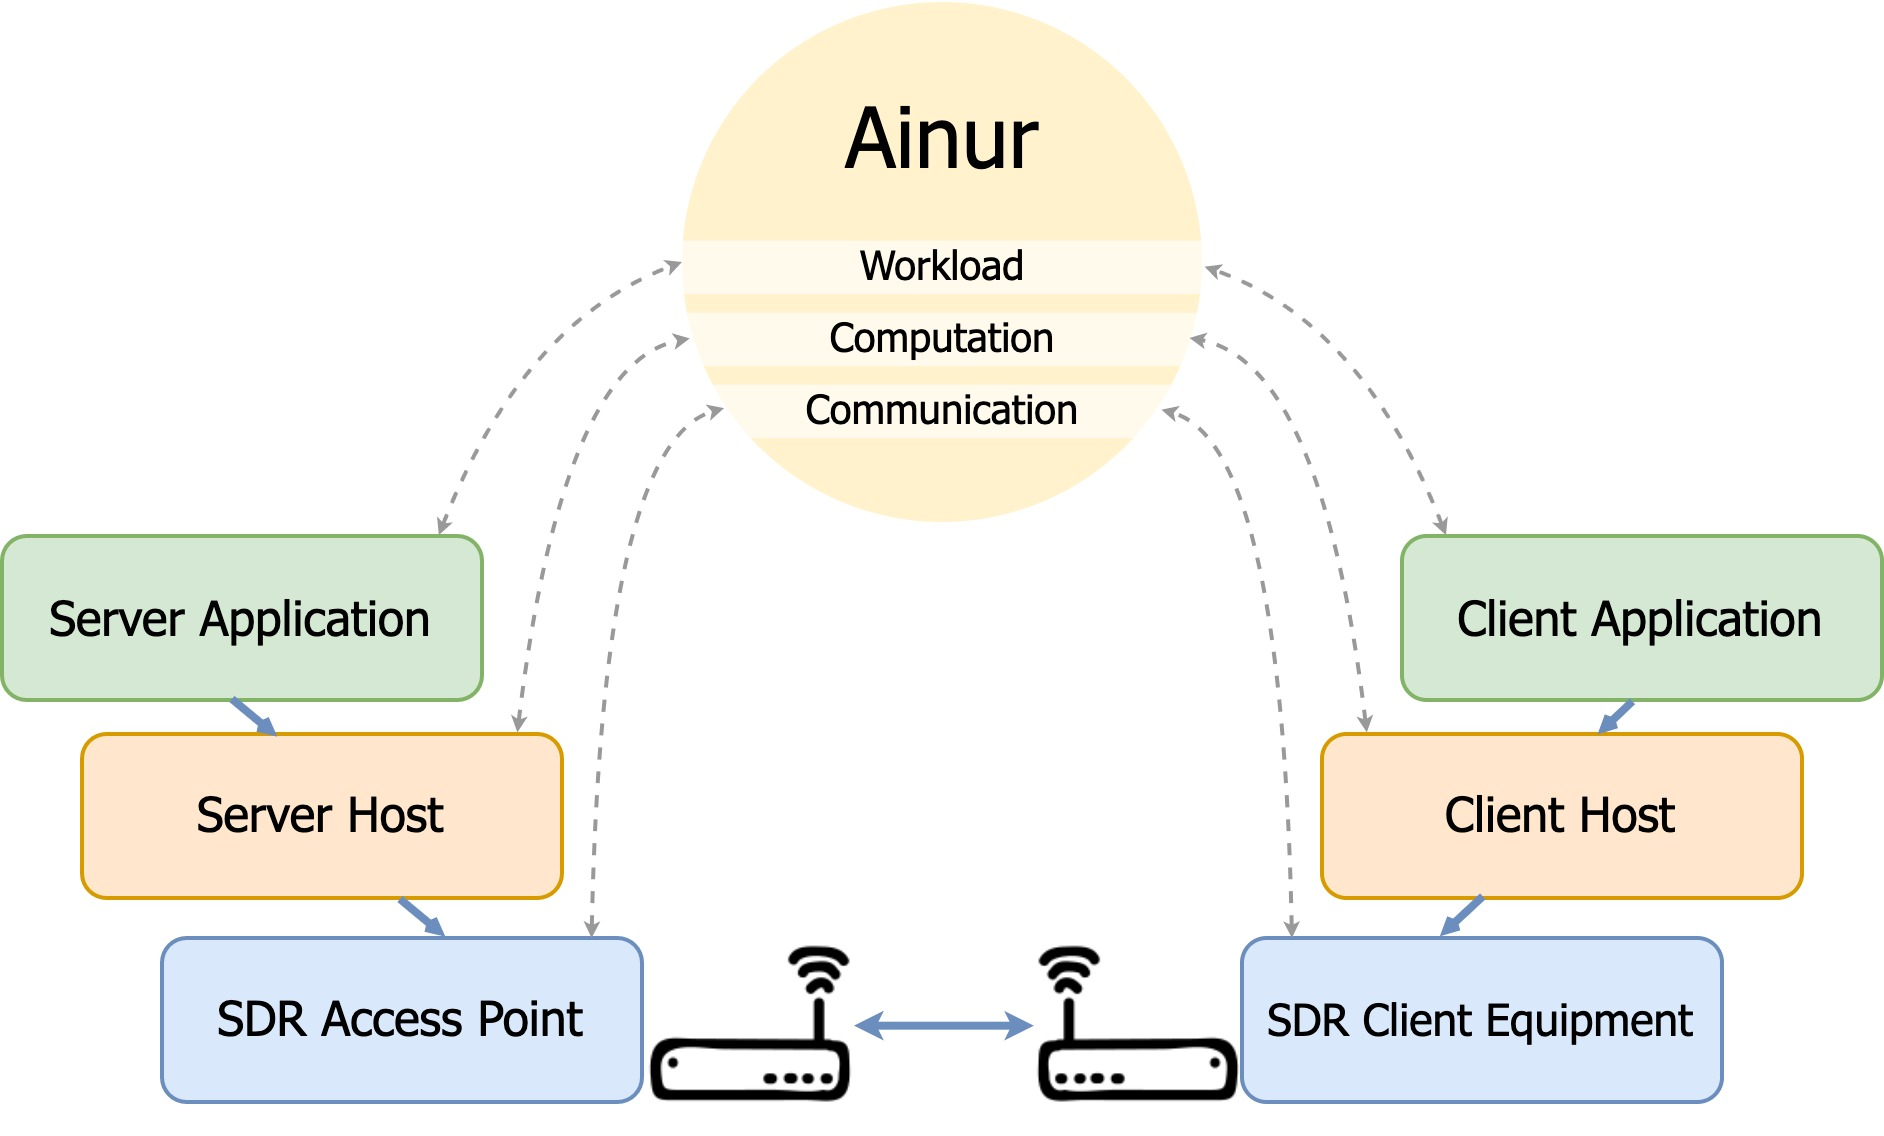
\includegraphics[width=0.9\linewidth]{publications/2022Ainur/figures/overview.jpg}
    \caption{Layered structure of an Ainur experiment}\label{fig:overview}
\end{figure}

\begin{figure*}
    \centering
    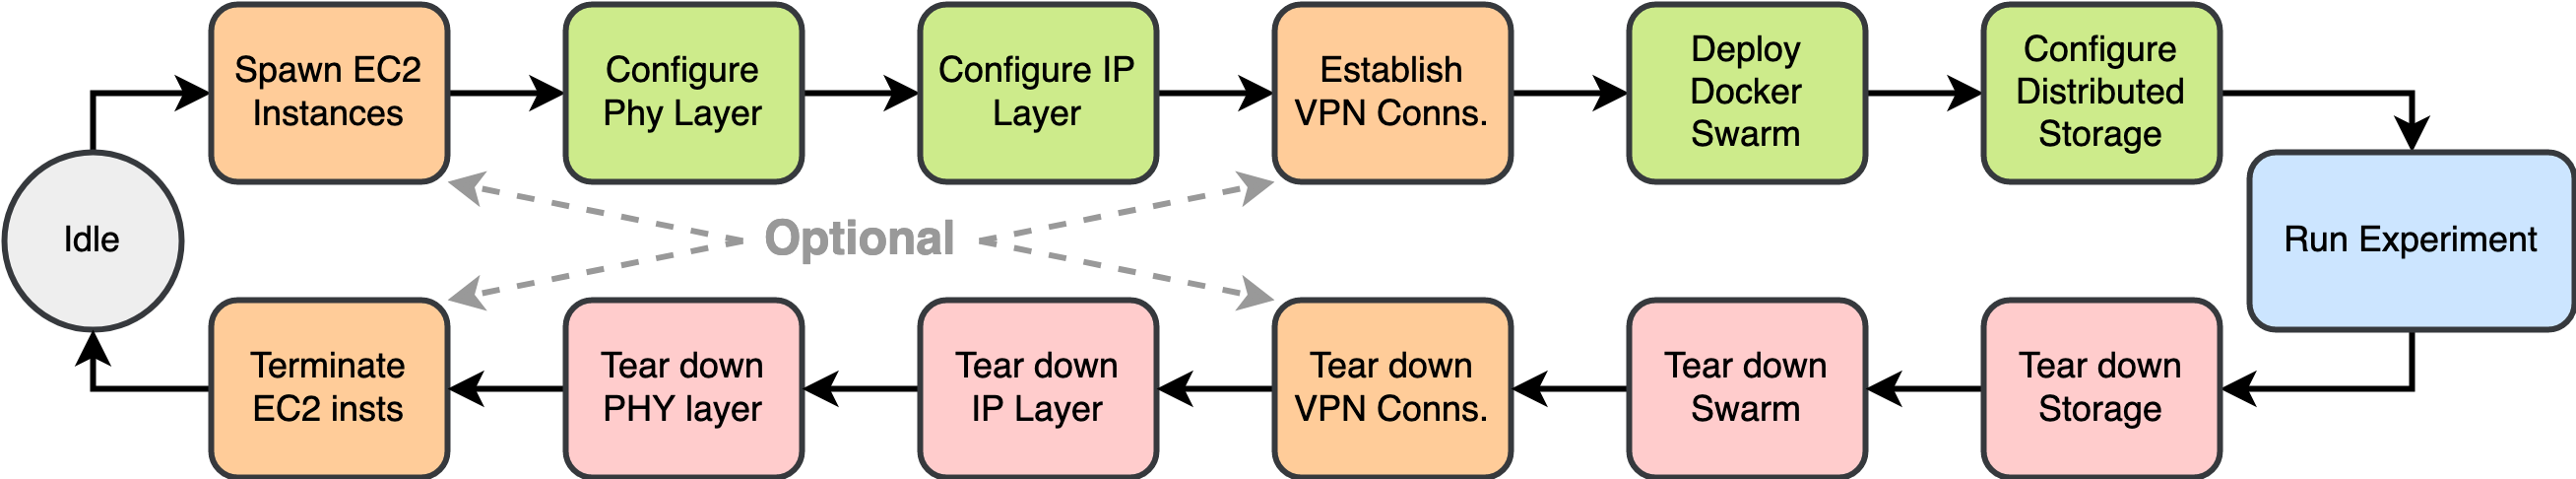
\includegraphics[width=0.8\textwidth]{publications/2022Ainur/figures/flow2.png}
    \caption{Lifecycle of an experimental run in Ainur. Blocks in orange are optional.}\label{fig:flow}
\end{figure*}

\begin{figure*}
    \centering
    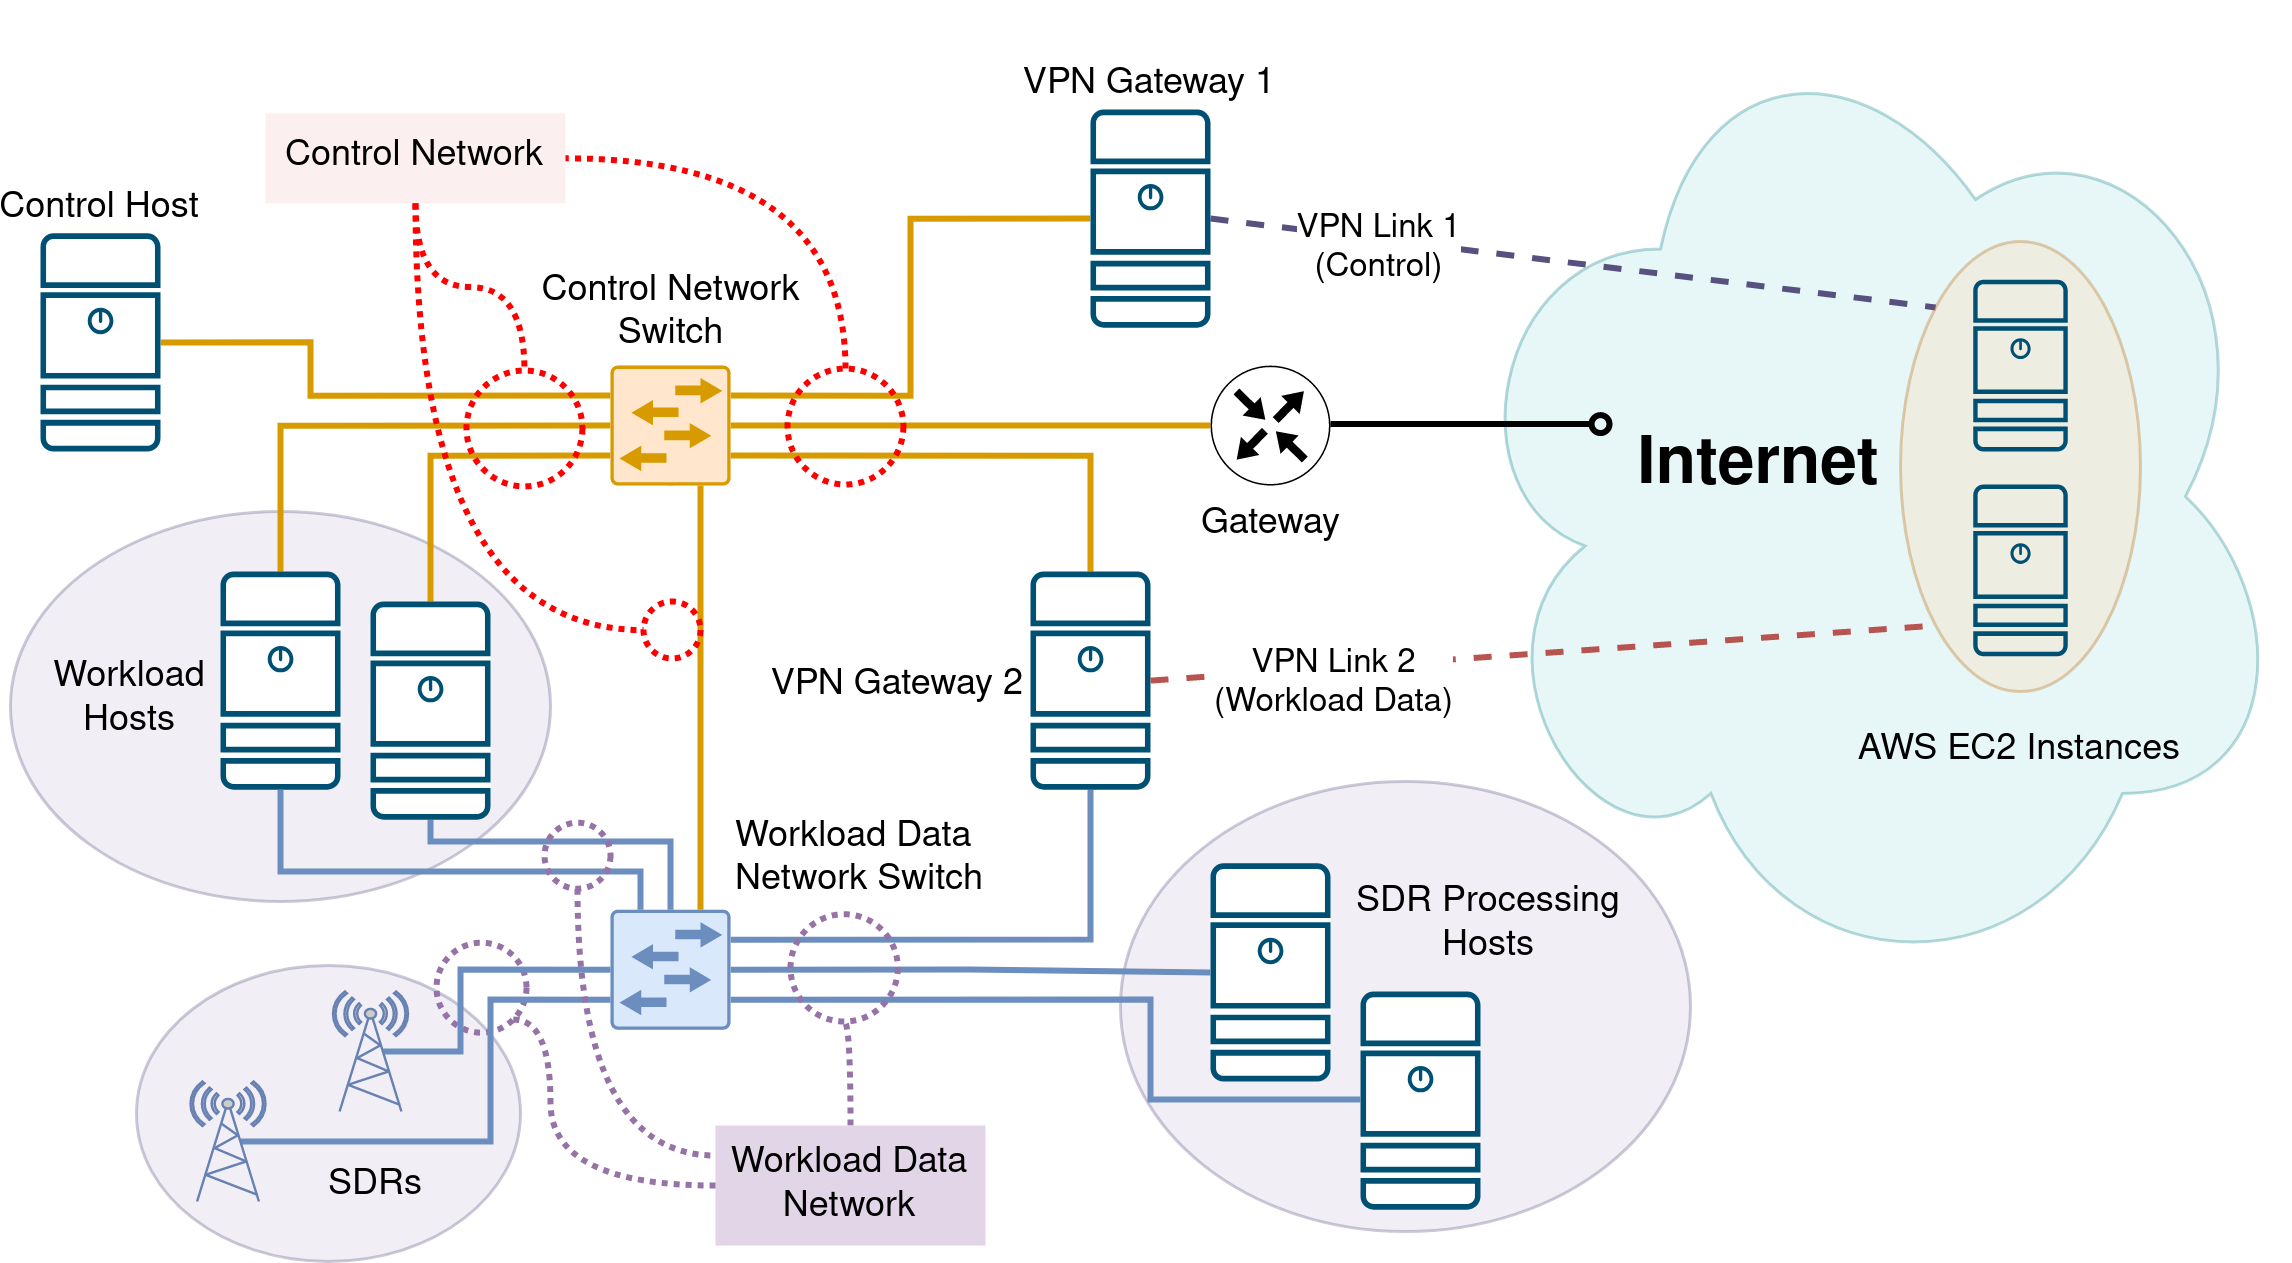
\includegraphics[width=.8\textwidth]{publications/2022Ainur/figures/network.png}
    \caption{Network structure assumed by Ainur.}\label{fig:network}
\end{figure*}

Ainur is designed as an end-to-end wireless network testbed management framework, fully flexible in terms of the communication network stack, computation hosts, and the distributed application deployed on top.
The core goal of the framework is to facilitate the creation of the desired communication and computation elements to discover their implications to the performance of end-to-end distributed applications.
Ainur achieves this by offering a Python \ac{API} which is used to describe an end-to-end experiment in a procedural manner, and we plan to eventually provide toolkits for declarative configuration of experiments.

Conceptually, in Ainur, an experiment is decomposed into a layered structure, consisting of
\begin{enumerate*}[itemjoin={{; }}, itemjoin*={{; and }}]
    \item the distributed application (workload)
    \item computation hosts
    \item communication networks connecting the hosts
\end{enumerate*}.
In \cref{fig:overview}, the workload is represented by a client-server process pair.
These could correspond, for instance, to the emulation of an inverted pendulum and a matching controller.
However, Ainur makes no assumptions about the nature of the workloads deployed on the framework, and virtually any process or combination of processes can be used.

Hosts correspond to either bare-metal machines or cloud instances on \ac{AWS} \ac{EC2}.
Users are free to combine and interconnect these in any configuration.
Ainur can provision wired networks over ethernet, and supports a number of software-defined wireless communication stacks, currently including WiFi, 4G \ac{LTE}, and 5G.
To realize these various wireless communication protocols, it is assumed that the testbed is equipped with \ac{USRP} \ac{SDR}s and some computation hosts dedicated to signal processing and/or radio management.

To collect data from workloads, Ainur configures both a shared, distributed, storage location which all processes can reach, as well as a logging service which automatically captures structured and unstructured data from the standard output of workload processes.
The logging service additionally collects data from the other two layers, and the resulting dataset could, for instance, be analyzed to relate the performance of the control loop to the quality of the wireless link. 

\subsection{Ainur Software Stack}

To realize our vision for an automated, flexible, cloud-native, and workload-agnostic framework for cloud and edge computing experimentation, we built Ainur on top of a combination of well-established tools and frameworks.
Below we briefly touch on the most important of these:

\begin{description}
    \item[Python:]
    Ainur is built on-top of Python 3.8.
    We chose this language for its flexibility, ease of prototyping, and for the extensive ecosystem of third-party cloud-native frameworks and libraries.

    \item[Ansible:]
    One of the ``cloud-native frameworks'' mentioned above, Red Hat Ansible is a powerful Python framework for bare-metal configuration, provisioning, and automation.
    We use it extensively in Ainur for configuration of network interfaces and services on managed hosts.

    \item[Containers:]
    We leverage Docker containers to great extent for the virtualization and orchestration of workloads, as well as the encapsulation and management of complex network configurations.
    See \cref{ssec:containers} for more details.    

    \item[\ac{AWS} and \texttt{boto3}:]
    Ainur employs the Amazon \texttt{boto3} library for Python to directly interface with \ac{AWS} \ac{EC2} and deploy, configure, and manage remote cloud instances.
    
    \item[\ac{OAI}:]
    \ac{OAI} is an open-source project that implements 3GPP technology on general purpose \texttt{x86} computing hardware and off-the-shelf \acp{SDR} like the \ac{USRP}~\cite{KALTENBERGER2020107284}. 
    Ainur can deploy, configure, and manage \ac{OAI} software components that implement 4G \ac{LTE} and 5G \ac{NR}.
    
    \item[Mango Communications 802.11:]
    Finally, the Mango Communications project implements real-time 802.11 (WiFi) MAC and PHY in Xilinx \acp{FPGA}.
    It can be used on a variety of hardware platforms including \ac{USRP} \acp{SDR}, and is employed in Ainur to provision end-to-end WiFi links.
\end{description}

\subsection{Main Software Components}

Ainur follows a layered architecture which closely mimics the conceptual layers of the \acs{TCP}/\acs{IP} stack.
Components are deployed in bottom-up order, starting with the establishment of physical links, through the establishment of \ac{IP} connectivity and deployment of links to the cloud, and ending with the distribution and initialization of workloads on top of a container orchestration layer.
The architectural modules of the framework can broadly be classified according to the below categories:

\begin{description}[]
    \item[Configuration Layer:]
    The lowest layer of Ainur. It handles the parsing of configuration files describing experimental scenarios.
    Optional, as it is only needed when Ainur is running experiments described in a declarative manner.

    \item[Logging layer:]
    This layer handles logging across all layers of the system to a central repository.
    Concretely, it manages the configuration and lifecycle of a Fluentd server to which any component in the network can send logs.
    Currently, the two main components relying on this scaffolding are the physical layer and the workloads.
    
    \item[Physical Layer:] 
    Creates and deploys the underlying physical connections of the workload data network.
    This layer interacts with hardware such as managed switches and \acp{SDR} (and their associated computation hosts) to create links between the desired workload hosts.
    These links correspond to ethernet, WiFi, and even an entire software-defined 4G \ac{LTE} and 5G networks.

    \item[Cloud Layer:]
    Handles integration with cloud services (currently, \ac{AWS} \ac{EC2}). 
    Only deployed in the case of an experiment requiring cloud instances, it manages the instantiation and configuration of remote cloud resources.

    \item[\ac{IP} Layer:]
    Configures and establishes \ac{IP} layer connectivity of packets between hosts in the experimental setup, both local and cloud.
    This includes assigning valid \ac{IP} addresses to hosts, establishing \ac{VPN} routes to cloud instances through a pair of pre-configured \ac{VPN} gateways, and configuring routing tables to ensure any two hosts in the workload network can communicate with each other.

    \item[Workload Layer:]
    Finally, this layer deploys, scales, and orchestrates containerized workloads, as well as configures a shared, distributed storage for workloads to store data.
    This components leverages Docker Swarm to spin up and manage workload containers on desired hosts.
    It also establishes overlay networks abstracting away the physical topology and allowing containers to interconnect through dynamically assigned hostnames.
\end{description}

\subsection{Containerization}\label{ssec:containers}

Containers are a key cloud-native technology for the virtualization and sandboxing of arbitrary processes~\cite{merkel2014docker}.
They allow for easy packaging of software in predefined, consistent, and conflict-free execution environments, including all necessary dependencies.
Containers are lightweight and portable compared to \ac{VM}-based virtualization, making them an ideal solution for the distribution, deployment, and orchestration of software in distributed computing environments.
They deploy quickly and are very configurable, while abstracting away the complexities and delays that come with in creating, managing, and moving (potentially huge) \ac{VM} disk images.

Ainur leverages containerization extensively across the framework, in order to
\begin{enumerate*}[itemjoin={{, }}, itemjoin*={{, and }}]
    \item deploy and orchestrate workloads
    \item support a wide spectrum of different physical layer configurations out-of-the-box, as well as allow for easy extension to new ones
    \item support automated collection of logs
\end{enumerate*}.
Workloads in the framework are deployed packaged in Docker containers, orchestrated through \texttt{docker-compose} and Docker Swarm.
We have selected Docker Swarm as our container orchestration layer instead of more advanced toolkits such as Kubernetes due to
\begin{enumerate*}[itemjoin={{; }}, itemjoin*={{; and }}]
    \item it being more lightweight
    \item its comparative simplicity in terms of configuration and setup
    \item the fact that it is included in the default Docker runtime installation
\end{enumerate*}.
This allows the framework to remain mostly agnostic to the nature of the workloads, and thus support a wide ranged of different applications and system architectures.
It also allows for easy deployment to different compute nodes in the network, without having to take into consideration details such as required libraries and versions.

As expressed above, Ainur also leverages containers for the communication stack.
With the advent of \ac{O-RAN} and \acp{SDR}, all components of the wireless network stack can run on general-purpose processors.
They can thus be containerized and distributed across multiple hosts.

As a final point, the automation of logging is another advantage of using containers and an orchestration framework.
Ainur employs the Fluentd unified layer for log collection.
It natively integrates with Docker containers and allows for the automatic collection of text data from the standard output and error streams of processes executing inside containers.
It automatically decouples data sources from containers running on different systems and allows Ainur to collect and classify the logs from any components of the network, whether on the wireless stack or workload.

\subsection{Obtaining Ainur and deploying it on a new testbed}

\begin{figure}
    \centering
    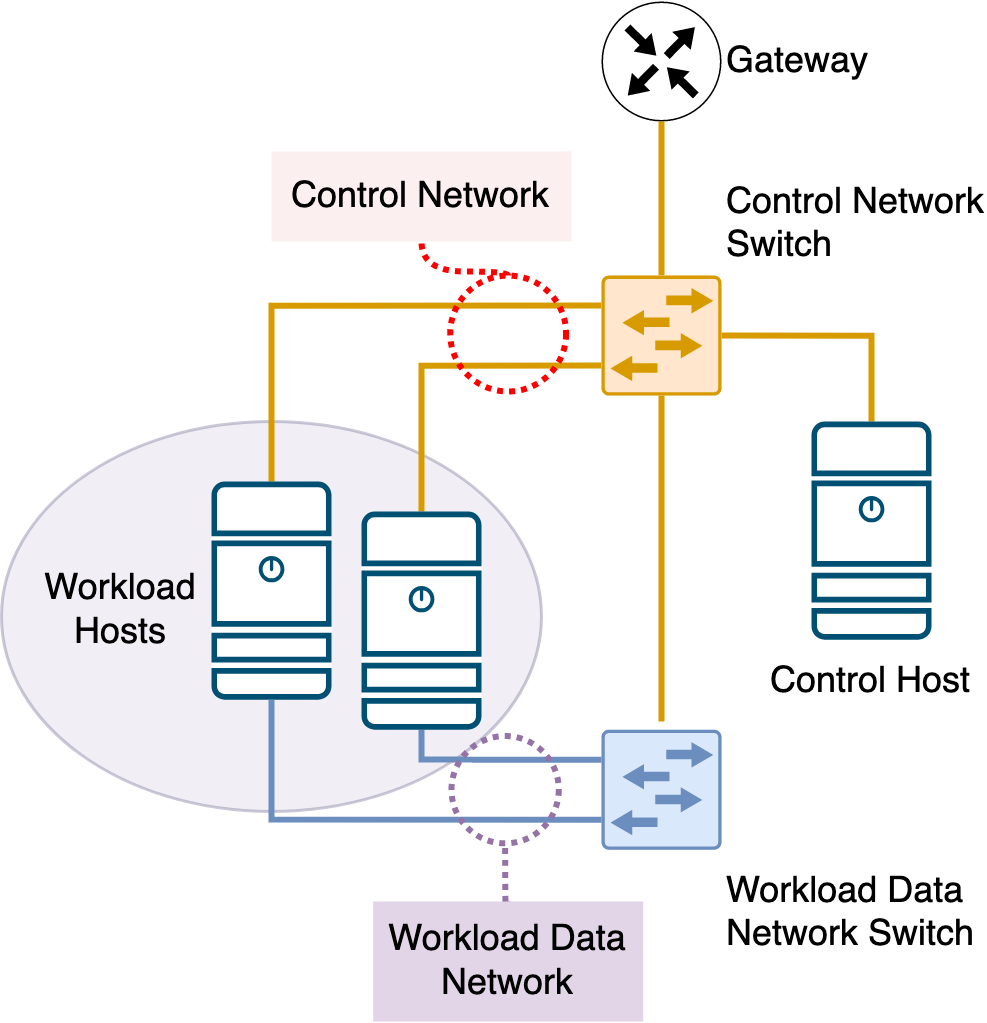
\includegraphics[width=.8\columnwidth]{publications/2022Ainur/figures/network-minimal.png}
    \caption{Minimal testbed setup on which Ainur can be deployed.}\label{fig:network:minimal}
\end{figure}

The framework is released as \acl{FOSS} under a permissive Apache license.
It can be downloaded from the Ainur repository~\cite{ainur:github} of the {KTH-EXPECA} organization on GitHub.
Given the software's complexity, the repository also includes detailed documentation on its requirements, configuration, deployment, and execution, as well as links to external resources containing information and guides about related concepts and services.

Ainur makes a number of assumptions about its execution environment.
Apart from generic ones regarding the presence of necessary authentication information for remote access to local and remote hosts and services, the framework assumes a split network architecture.
Ainur runs in a dedicated control host and the management plane resides in a physically distinct network from the workload data.
This is a key requirement to be able to reconfigure the physical links in the workload data network without disrupting management traffic.

A full-featured, and rather complex deployment is depicted in \cref{fig:network}, including a number of optional testbed features such as offload to the cloud through \ac{VPN} gateways.
However, a minimal a setup can be achieved with a control host, at least two workload hosts, and a couple of managed (smart) switches, as illustrated in \cref{fig:network:minimal}.
The only requirements for the aforementioned hosts are that a general purpose Linux distribution such as Ubuntu can be deployed on them, and --- in the case of the workload hosts --- the presence of two network interfaces.
Thus, a minimal testbed can be achieved cheaply and quickly by employing small single-board computers such as Raspberry Pi, Jetson Nano, or BeagleBone units.
Finally, the configuration and deployment of an Ainur-compatible testbed can be easily automated with tools such as Ansible, and playbooks for this effect can be made available to the community upon request.

% Also assumed is the existence of \ac{VPN} gateways to the cloud, time synchronization, and configured hostname lookups (possibly using a \ac{DNS} service).



\begin{figure*}
    \centering
    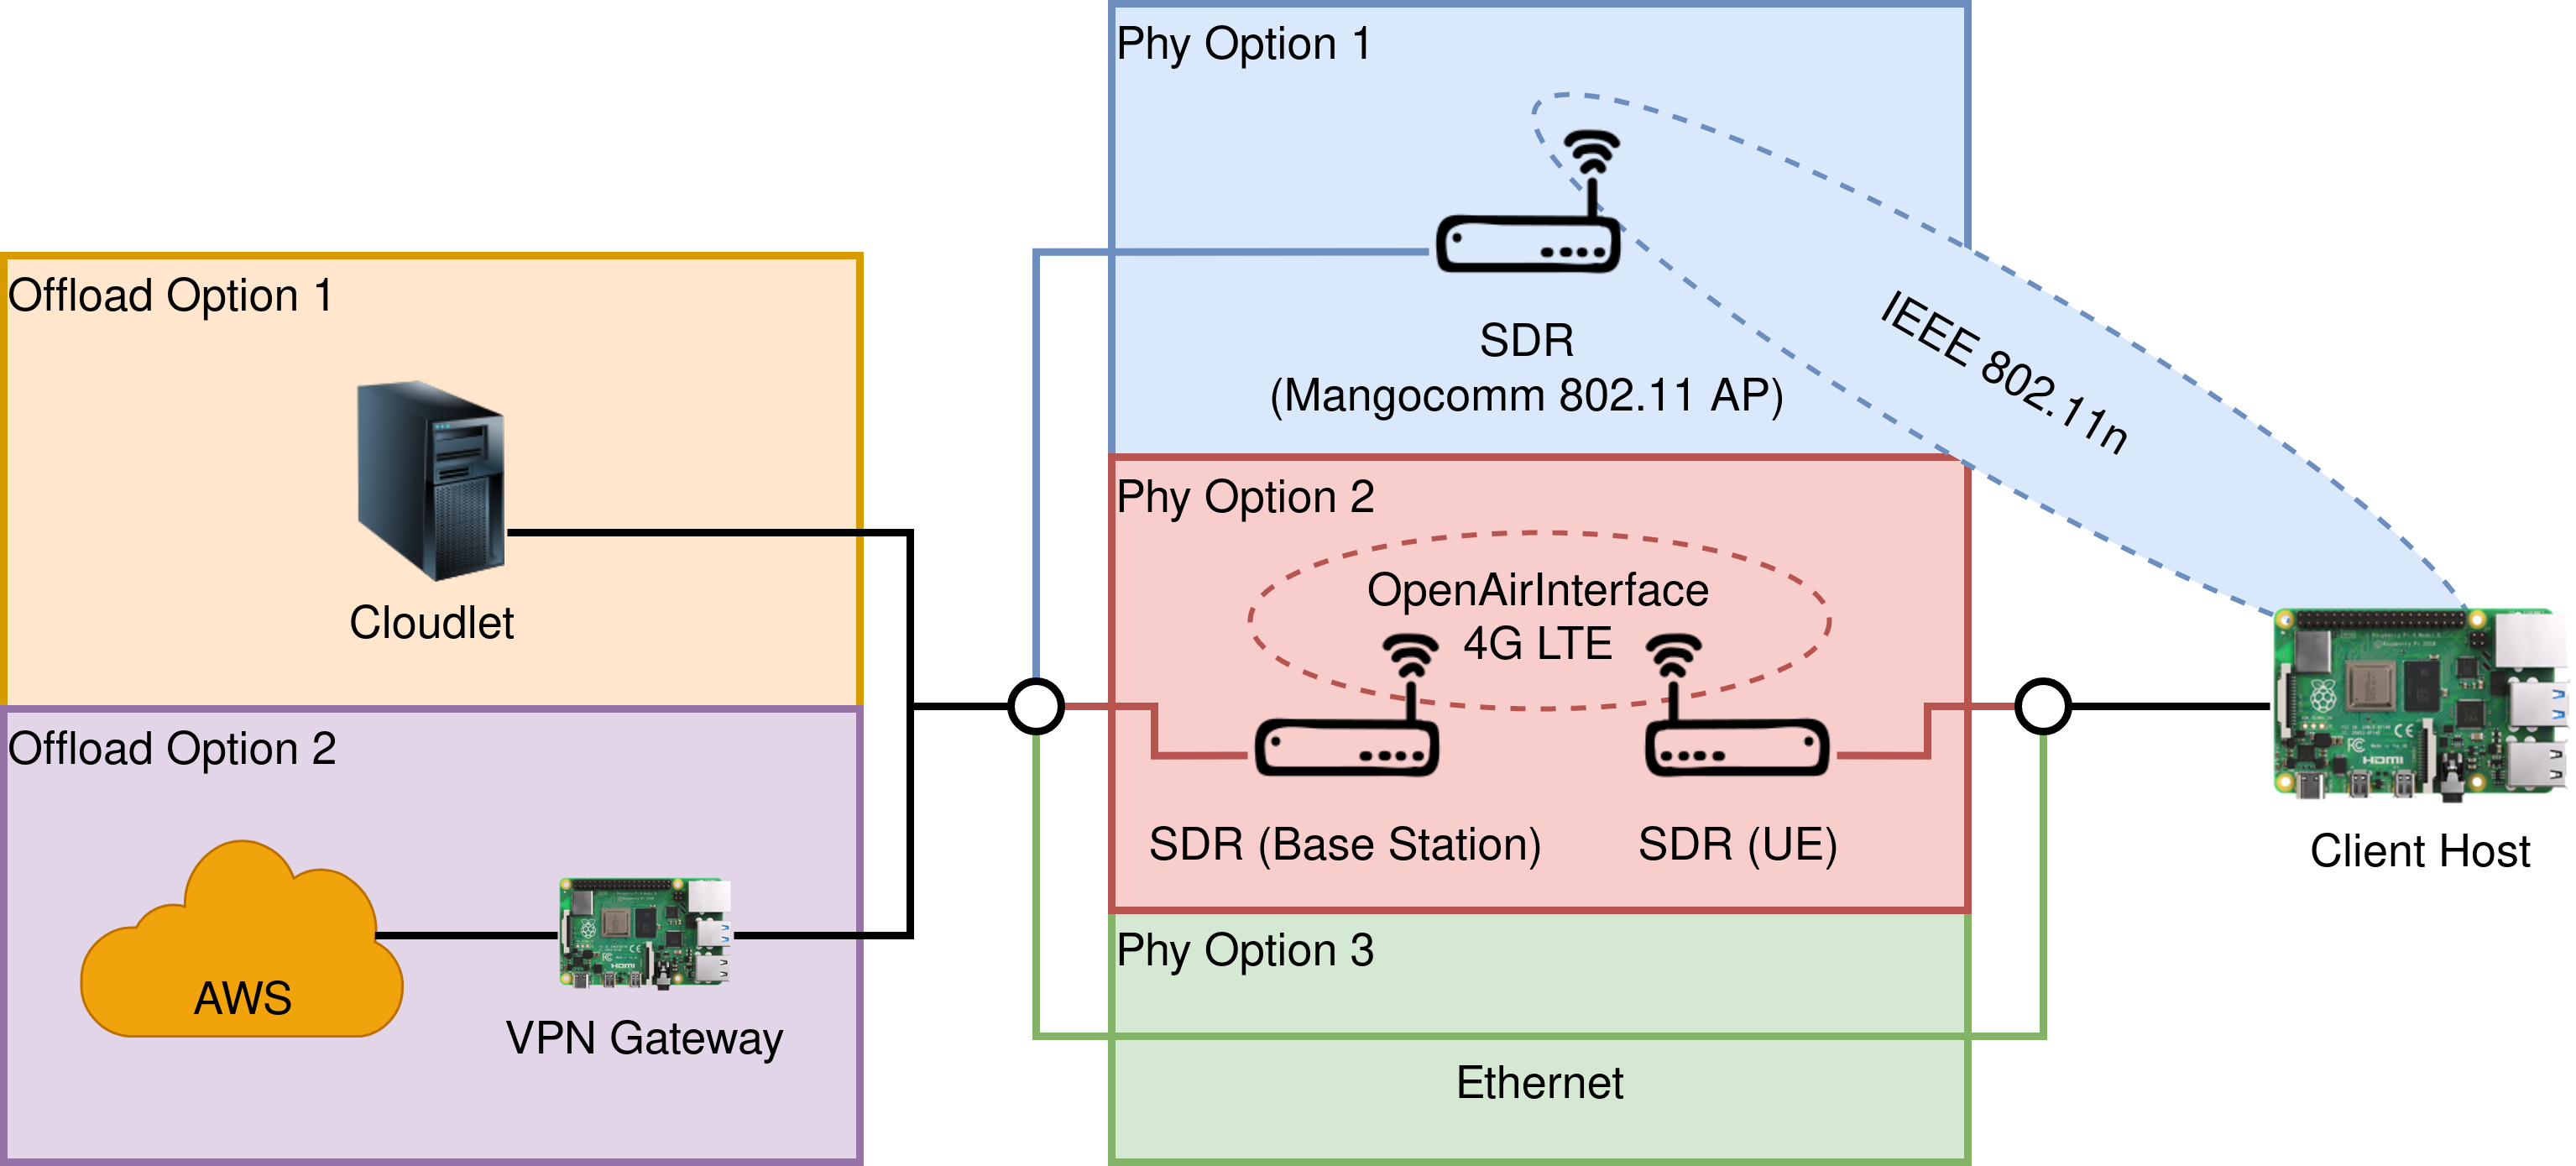
\includegraphics[width=.8\textwidth]{publications/2022Ainur/figures/demo_hardware.png}
    \caption[caption]{%
        The possible workload offloading setups and physical layer configurations used in the demo.
        Not pictured, in Phy Option 2:
        \begin{enumerate*}[itemjoin={{; }}, itemjoin*={{; and }}]
            \item \ac{SDR} processing hosts 
            \item additional base-station host for the Core Network and \ac{eNodeB}
        \end{enumerate*}.
    }\label{fig:democonfigs}
\end{figure*}

\begin{figure}
    \centering
    \begin{subfigure}{\columnwidth}
        \centering
        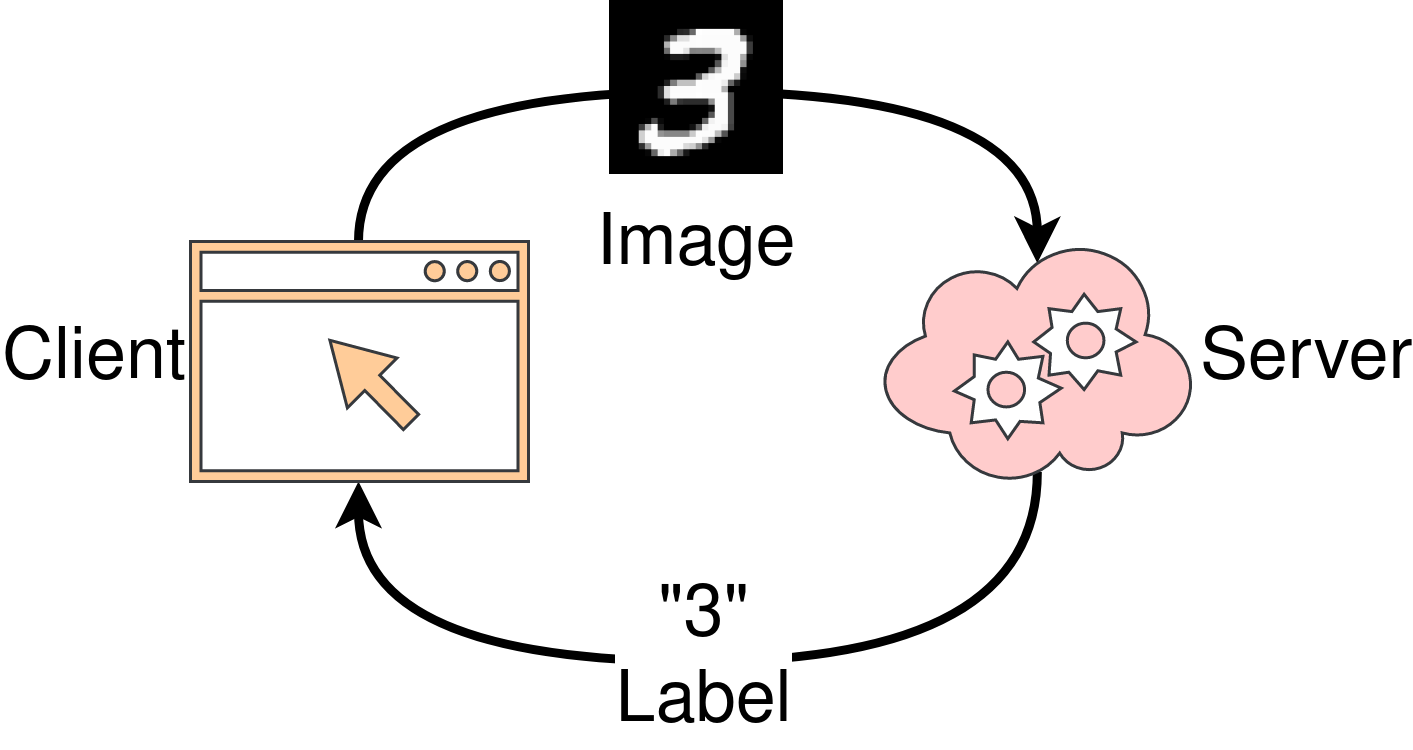
\includegraphics[height=8em]{publications/2022Ainur/figures/demo_workload_1.png}
        \caption{Workload 1: \acs*{MNIST} image classifier}\label{fig:wkld:mnist}
    \end{subfigure}%
    \vspace{1em}
    \begin{subfigure}{\columnwidth}
        \centering
        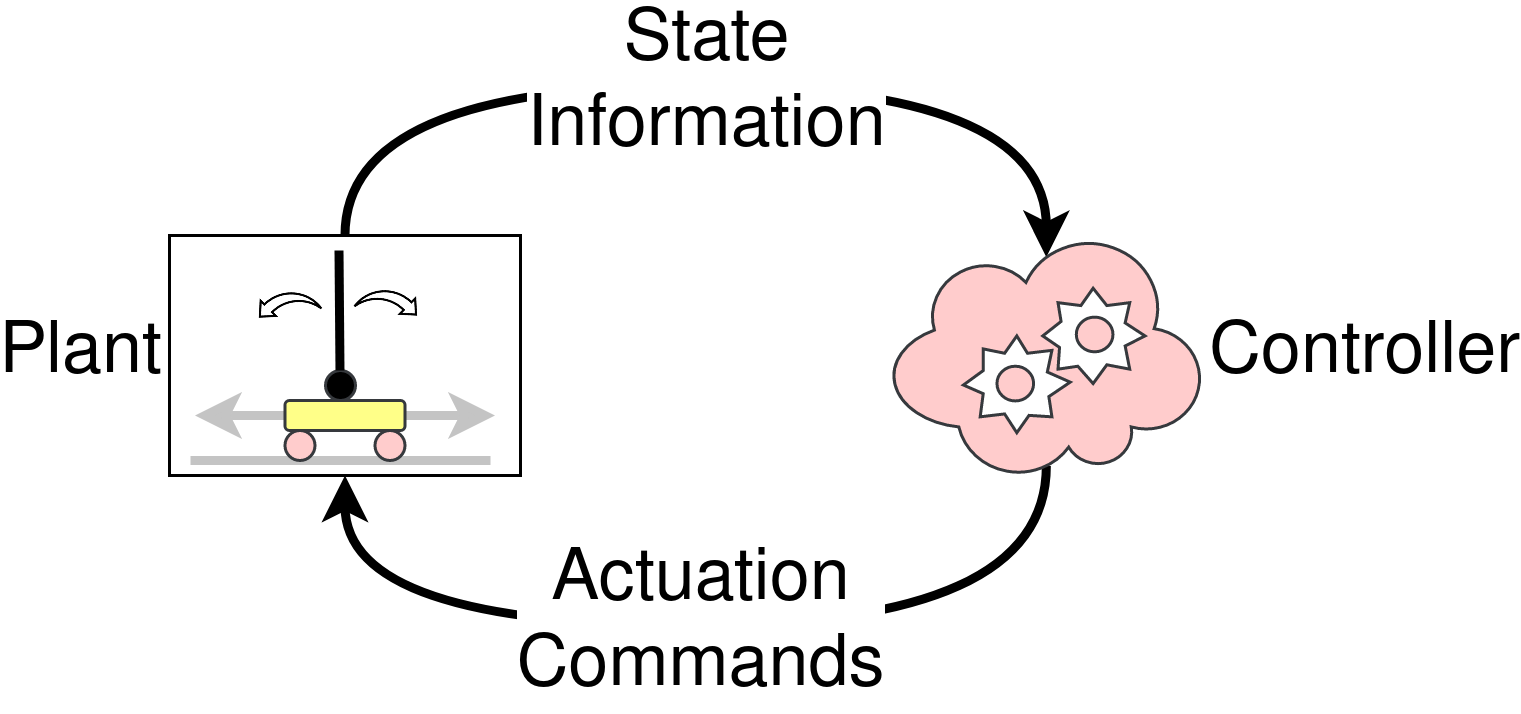
\includegraphics[height=8em]{publications/2022Ainur/figures/demo_workload_2.png}
        \caption{Workload 2: inverted pendulum \acs*{NCS}}\label{fig:wkld:ncs}
    \end{subfigure}
    \caption{Demonstration workloads}\label{fig:wkld}
\end{figure}

\section{Demo}\label{sec:demo}

In this demo, we will show the flexibility of Ainur for running end-to-end experimental workloads on both the Edge and the Cloud.
This will be done interactively, and members of the audience will be invited to propose testbed configurations.

\Cref{fig:democonfigs} illustrates the possible configurations for the testbed.
Workloads are deployed on client hosts, and computation is offloaded either to an edge server (cloudlet), or to \ac{AWS} \ac{EC2} instances on the cloud.
Communication between the client- and server-sides of the workload will occur over one of three possible physical link layer setups:
\begin{description}
    \item[WiFi:] \iac{SDR} is configured as an IEEE 802.11n access point, and client hosts connect to it using on-board WiFi.
    \item[4G \ac{LTE}:] \iac{SDR} is configured as an 4G \ac{LTE} base station, and another is configured as an 4G \ac{LTE} \ac{UE}.
    Together these radios act as an \ac{LTE} bridge between the client-side and the server-side of the network, and all client-server traffic is routed through them.
    \item[Ethernet:] connects everything through plain ethernet.
\end{description}

The number of workload instances (and therefore client hosts) deployed in each execution of this demonstration will range from \numrange[]{1}{10}.
Workloads deployed to the cloud will be able to target any of \ac{AWS}'s datacenters.

We will employ two different workloads for this demonstration, illustrated in \cref{fig:wkld}.
The first of these (\cref{fig:wkld:mnist}) consists of a proof-of-concept web application which implements a simple classifier to identify hand-drawn digits from the widely-used \ac{MNIST} dataset~\cite{mnist}.
The application consists of a client with a web interface, and \iac{HTTP} server which responds to requests from the client and performs the actual image recognition.
This workload is intended to showcase in an interactive manner the effects of placing computation at different points of the network, and how Ainur simplifies these deployments.

The second workload (\cref{fig:wkld:ncs}) corresponds to \iac{NCS} balancing an inverted pendulum, implemented on a software framework for the emulation of \acp{NCS} using cloud-native technologies~\cite{cleave}.
It consists of an emulation of the physical inverted pendulum system plant and a software-implemented proportional-differential controller.
These components communicate with each other over the \ac{UDP}.
This workload will be used to showcase the utility of Ainur for automating the execution of batches of experiments potentially including multiple different clients, servers, and physical layers.

\subsection{Testbed Setup}

This demonstration will be performed on a testbed consisting of
\begin{enumerate*}[itemjoin={{; }}, itemjoin*={{; and finally }}]
    \item \num{10} Raspberry Pi 4 Model B boards, acting as client-side workload hosts
    \item a Raspberry Pi 4 Model B acting as \ac{VPN} gateway for the workload network
    \item a Raspberry Pi 4 Model B acting as \ac{VPN} gateway for the management network, as well as hosting the necessary \ac{NTP} and \ac{DNS} server software
    \item a \texttt{i386} workstation, acting as an edge-side workload host
    \item a configurable number of  \ac{AWS} \ac{EC2} cloud instances acting as cloud servers
    \item a separate \texttt{i386} workstation hosting the Fluent server and on which Ainur is deployed as well.
\end{enumerate*}
These nodes are interconnected using a combination of managed switches, \acp{SDR}, and \ac{VPN} gateways; please refer to \cref{fig:network} for an architectural overview of this setup.


\subsection{Demo Procedure}

\subsubsection{Workload 1}

\begin{figure}
    \centering
    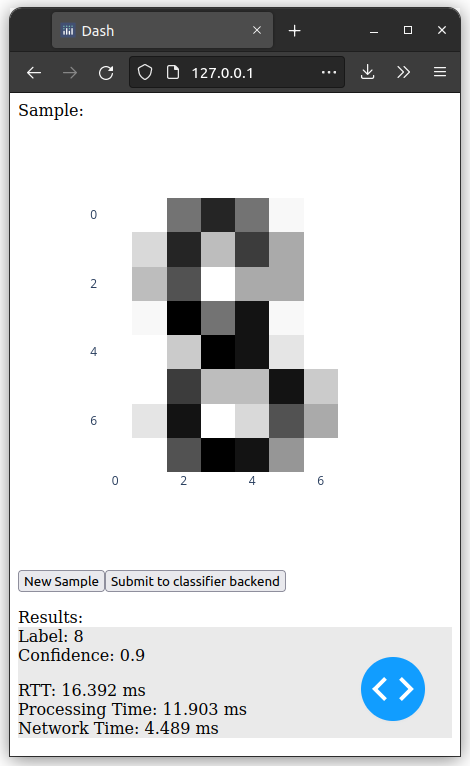
\includegraphics[width=.65\columnwidth]{publications/2022Ainur/figures/demo_mockup.png}
    \caption{Screenshot of the user interface of demo workload 1. After deciding on the placement of the compute backend and the type of physical layer connecting client and backend, participants will use this interface to interact with the system.}\label{fig:mockup}
\end{figure}

Participants will be asked to choose
\begin{enumerate*}[itemjoin={{; }}, itemjoin*={{; and }}]
    \item a location to offload computation to (local (i.e.\ no offloading), edge, or any \ac{AWS} datacenter)
    \item a physical layer for the first hop of the network (WiFi, 4G \ac{LTE}, or ethernet). 
\end{enumerate*}
Through the Ainur command line, we will deploy a single client-server pair according to the specifications.
Next, participants will be able to access the client web interface and interact with the server by requesting classification of images from the \ac{MNIST} database.
The server will respond to these, and the assigned labels will be visible on the web interface together with timing statistics for each request, see \cref{fig:mockup}.

\subsubsection{Workload 2}

Participants will be asked to specify the full, arbitrarily complex, experimental scenario, including the number of clients, physical layers (single or multiple, and which clients are on each physical link), and offloading configuration (number of instances on the edge vs.\ on the cloud, which \ac{AWS} datacenters to deploy to).
Configuration will be specified through a \acs{YAML} file, which will then be parsed by Ainur for the automatic execution of the scenario.
\section{Conclusion}\label{sec:conclusion}

The issue of repeatable and scalable benchmarks has been largely glossed over in \ac{NCS} literature, as existing experimental research studies tend to implement \emph{ad-hoc} solutions.

In this work, we aimed to tackle this issue through a fully software-based framework for repeatable, reproducible, and easily scalable \ac{NCS} benchmarking with a particular focus on edge deployment.
We argue our approach, \ac{CLEAVE}, embodies a better solution than previous work for a number of reasons:
\begin{enumerate}
    \item Compared to fully physical approaches, such as those used in\ \cite{Baumann2018LowPower} and\ \cite{Cuenca2019UAV}, our approach allows for greater flexibility and scalability.
    The aforementioned approaches rely on specialized and sometimes entirely custom-built physical platforms, and although flexible and cheap approaches such as Zoppi \emph{et al.'s} --- which uses a LEGO-based physical plant --- exist, these still do not reach the level of flexibility afforded by a fully software-based framework. 
    Experimenters still need copies of the hardware, making anything other than small-scale setups unfeasible.
    In contrast, our approach requires only general-purpose computing platforms, and can be employed by basically anyone with access to a computer.
    Scalable deployments can in turn easily and cheaply be set up using single-board computers and/or virtual cloud instances.
    \item When compared to simulated approaches such as\ \cite{Ma2019DynamicSched}, \ac{CLEAVE} provides a higher level of realism, in particular with regards to the network segment of the system.
    \item Finally, although it shares much in common with previous emulated approaches such as the one employed in\ \cite{Wang2020VoltageControl}, \ac{CLEAVE} has an advantage by specifically targeting a general-purpose approach using industry-standard, cloud- and edge-native tools and software.
    The tool can easily be deployed and scaled using widely-used frameworks such as Docker Swarm and Kubernetes.
\end{enumerate}

We validate the utility of this tool through an example use case approximating a proposed edge deployment of inverted pendula control loops co-located with video analytics services.
We argue such a use case represents a realistic scenario and appropriate benchmark for the tool, since
\begin{enumerate*}[itemjoin={{; }}, itemjoin*={{; and }}]
    \item the inverted pendulum plant is ubiquitous in \ac{NCS} research
    \item similar setups exist in real-world industrial use
    \item video analytics has long been proposed as a ``killer app'' for edge computing.
\end{enumerate*}
Our results showcase the ability of the framework to extract relevant metrics relating to the stability of the control system, as well as on the performance of the underlying network link.
We believe \ac{CLEAVE} represents an important step towards enabling inexpensive and low-complexity scalable research for real-world deployment of edge-bound \acp{NCS}.

There is still, however, work to be done.
We are extending the number of plant and controller implementations on the framework, with the goal of creating an open library of \acp{NCS} to share with the community.
At the moment, the interactions of \ac{CLEAVE} and tools such as Docker are still quite superficial.
Our goal is to achieve a much tighter integration, e.g.\ by providing the toolkit as pre-packaged container images.
Finally, the validity of the results obtained by the framework will have to be verified through more thorough, realistic scenarios than what we have been able to show in this work.
In particular, we intend to perform large-scale experimentation targetting 5G cellular deployments, as this technology is set to become the backbone of edge networks in the near future.

%%%%%%%%%%%%%%%%%%%%%%%%%%%%%%%%%%%%%%%
%%%%%%%% ACKNOWLEDGMENT %%%%%%%%%%%%%%%
%%%%%%%%%%%%%%%%%%%%%%%%%%%%%%%%%%%%%%%
\chapter{Acknowledgements}
\epigraph{La educación es, tal vez, la forma más alta de buscar a Dios.}{\emph{Gabriela Mistral}}
\glsresetall%

There are many, many people I owe gratitude to for making this dissertation possible.
I would like to begin by thanking my supervisor, Prof. James Gross.
This dissertation would not have been possible without his guidance and motivation during this long process.
His supervision opened doors that I had never imagined would open for me, and his dry German humor has certainly helped cheer me up whenever I was overwhelmed by some deadline.
Above all, I would like to thank James for his patience and understanding whenever I encountered difficulties, and for the flexibility he has afforded me in completing this Ph.D.

I would like to express my deepest gratitude to Prof. Mahadev ``Satya'' Satyanarayanan, for welcoming me repeatedly, over long periods of time, as a visiting researcher at \gls{CMU}.
Likewise, I'm deeply indebted to Prof. Roberta ``Bobby'' Klatzky of \gls{CMU} for the many helpful and insightful discussions, for introducing me to the field of Human-Computer Interaction, and for always greeting me with a warm smile.
Both Satya's and Bobby's tremendous experience and generosity have been invaluable, and their guidance and advice have certainly shaped my work for the better.

I would also like to thank everybody involved with the defense of this thesis.
I am very grateful to Prof. Yu Xiao of Aalto University, for agreeing to act as my dissertation opponent.
My dissertation defense will certainly benefit greatly from her expertise and insights.
I would like to extend my sincere thanks to my grading committe, consisting of Prof. Ana Aguiar (Universidade do Porto), Prof. Per Gunningberg (Uppsala Universitet), and Prof. Klaus Wehrle (\gls{RWTH}), for investing time and effort into reading and grading this dissertation.
Special thanks also go to Prof. Markus Flierl of \pgls{KTH} for advance-reviewing this dissertation, and to Prof. Mats Bengtsson, also of \pgls{KTH}, for agreeing to act as chairperson for the defense.

Moreover, I extend my thanks to my co-authors and colleagues.
To Samie Mostafavi, Vishnu N. Moothedath, and Neelabhro Roy at \pgls{KTH}, for always being willing to engage in interesting discussions, but also for generally being fun to be around.
And to Dr. Jaya Prakash (IMDEA Networks Institute), Dr. Junjue Wang (\gls{CMU}), and Dr. Padmanabhan ``Babu'' Pillai (\gls{CMU}) for enriching my research with their interesting insights.

I am very lucky and grateful that I got to stay at both \pgls{KTH} and \gls{CMU}, and I would like to thank everyone who made these spaces welcoming and engaging.
A big thank you goes out to my colleagues (both current and former) at the division of \gls{ISE} for all those fun lunches at Restaurang Q, Cypern, and SysterOBror over the years, which always helped to break the monotony of the days.
This includes but is not limited to Samie, Vishnu, Neel, Sahar, Antonios, Germán, Boules, Baptiste, Håkan, Pol, Marie, Wendi, and Sebastian.
I would additionally like to extend a special thank you to Dr. Sebastian Schiessl, for ``taking me under his wing'' when I first arrived at \gls{ISE} and acting as a sort of mentor during my first moths.
Likewise, I extend my gratitute to Gerd Fransson, for greeting me with a huge smile every morning the years our offices faced each other and cheering up my days with her wholesome energy.
I also thank Prof. Joakim Jaldén for giving me the opportunity to act as his teaching assistant.
Another big thank you goes out to everyone (current and former) at Satya's group at \gls{CMU}, for always welcoming me with open arms and treating me like one of them whenever I was visiting.
This includes but is not limited to Junjue, Tom, Roger, Shilpa, Jan, Edmond, Jim, Babu, and Zhuo.
I will always remember our Monday morning talks and Friday lunch outings dearly.

Furthermore, I would like to extend my sincere thanks to Prof. Sandra Céspedes, of Universidad de Chile and Concordia University, for her guidance and urging to embark on this journey towards a Ph.D., and for always being willing to offer help and advice.
Likewise, I'd like to thank Prof. Javier Bustos, of Universidad de Chile and NIC Chile Research Labs, for giving me the opportunity many years ago to first get into distributed systems research.
Also, I'd like to extend my gratitude to Prof. José Miguel Piquer, of Universidad de Chile, for taking me as his ``long-distance'' teaching assistant and allowing me to give back to my \emph{alma mater} from across the ocean.
A very special thanks goes out to Prof. Jérémy Barbay of Universidad de Chile and Universidad de Concepción, for being both a mentor and a friend since the day I took his course on Android programming as an undergraduate student.
I am deeply appreciative of the fact that although our interactions these last few years have been sporadic at best, I can always reach out to him for help and advice when I need them.

\medskip

This dissertation would not have been possible without the help and support of my family.
First and foremost, I would like to thank the love of my life and wife~\footnote{\emph{Future-wife} at the time of writing, but \emph{wife} at the time of the defense of this thesis!}, Andresa.
I could not have done this without her companionship and love.
I am eternally grateful for her unconditional support over difficult periods of time and over tremendous distances while we were living apart, and for making every day we spend together amazing.

I am also deeply grateful to my parents, Gabriel and Valeria, for always encouraging my curiosity and my drive to learn and discover.
They have been my rocks, my pillars, since the day I was born, and I am proud to be their son.
A big thank you goes out to my sister, Paola, as well.
Although we sometimes get on each other's nerves, she has always been there for me and supported me, and I could not have asked for a better sister.
Likewise, I extend my deepest gratitude to everyone in my immediate and extended family who have given me support and love over the years, including but not limited to my paternal grandparents, Manuel and María Yolanda, my maternal grandparents, Caupolicán and María Aura, my uncle Mauricio, his wife Marylen, their daughter Amanda, and everybody else.
I would like to make a special mention to my late grandfather, Caupolicán ``Poli'' Muñoz, who always inspired and fanned the flames of academic curiosity in me.
I hope he would have been proud seeing how far I have come.
Another special mention goes to my uncle Manuel, who graciously took me in and gave me a place to stay at the first few months of my Ph.D. studies.

I would also like to thank all of my friends who have made this long, ardous journey more amenable.
I would particularly like to thank everyone I met through Tartan Salsa, including, but not limited to, Andresa, Jennifer, Alyson, Kuai-Kuai, Carmen, Moataz and Nora, Eric, and many others.
They made Pittsburgh feel like home, even before I finally moved there permanently in 2022.
I also want to thank Ann-Charlotte in Stockholm, for always being so kind, so considerate, and so much fun to be around.
Further, I am deeply grateful to my friends in Chile who have remained a source of support, even though we only get to see each other once a year when I visit.
This includes, but is not limited to, Juan Pablo, Fernanda, Diego, Camila, George, Patricio, Kevin, Pablo, and many others.
Yet another special mention goes to Diego's family, who have always treated me as one of their own.

Finally, I would be remiss in not mentioning my pets and animal friends who have provided me with love and warmth during these years.
I thank my dogs, Aros and Skatt, who I sadly had to leave behind in Chile with my sister, but who still greet me with enthusiastically wagging tails whenever I visit.
And I thank my cats, Mochi and Tiramisú, who, although have only been in my life for about a year, have sweetened and made much more bearable the long days and nights I have spent writing this dissertation.

\bigskip

\noindent{}Manuel Olguín Muñoz\\
Pittsburgh, May 2023
% \section{Future Work (ExPECA 2.0)}

\begin{description}[wide,style=nextline]
    \item[Client-Server Architecture and Microservices]
    Our current design follows a monolithic approach, in which ``layers'' of software build upon each other to reach a desired state.
    This approach is easy to understand and somewhat straightforward to implement, and works well for end-to-end experimentation.
    However, it causes a couple of problems, for example:

    \begin{enumerate}
        \item Components in the implementation are quite tightly coupled, so adding new functionality or layers in many cases implies rewritting large chunks of code.
        This also requires quite a lot of synchronization between people working on different parts of the code.
        \item It makes experimentation synchronous, and when running things over \ac{SSH}, it requires the use of tools such as \texttt{screen} or \texttt{tmux} to be able to run long experiments without having to keep the connection open at all times.
        \item We currently have no way of ensuring mutual exclusion of multiple instances of Ainur on the testbed, and implementing such functionality would probably require some sort of centralized instance tracking mechanism.
    \end{enumerate}

    I (Manuel) suggest then that for ExPECA 2.0 we switch to a distributed client-server architecture, using a microservice for each core functionality.
    In other words, we would have several smaller server applications running on potentially different hosts on the network, each handling a specific part of the functionality we need.
    For instance, we could have a ``Layer 3'' service which handles setting up \ac{IP}-layer connectivity, and another ``SDR'' service which manages the \acp{SDR}.
    Services could communicate with each other using simple HTTP \acp{API} for easy debugging, and we would have an ``Ainur'' client which orchestrates the services into an experimental run.

    This has several advantages:

    \begin{enumerate}
        \item It decouples the implementation details for each service.
        As long as the \ac{API} is well-defined, it doesn't matter how the service is implemented - we could even use different languages for different functionalities.
        \item Adding new functionality becomes simply a matter of writing a new microservice and plugging it into the existing setup.
        \item Experimentation can be done asynchronously through an ``experiment scheduler'' service which queues, runs, and then collects results from experiments.
        This service would also then ensure mutual exclusion of testbed resources.
        \item Things could be parallelized.
        Our current design is sequential, even when it doesn't need to be.
        Things that do not depend on each other could be executed in parallel (e.g. cloud and local configuration), cutting down on experiment time overhead.
        \item It would fit squarely into the design of both Docker and Kubernetes, both of which are distributed client-service architectures.
    \end{enumerate}

    \item[OpenStack/Canonical MaaS]
    
    We should really consider switching to a mature framework for bare-metal provisioning instead of doing it manually with Ansible.
    Potential options are OpenStack Ironic and Canonical Metal-as-a-Service.

    \item[Raspberry Pi SSDs]
        
    Currently our Raspberry Pis boot Ubuntu 20.04 LTS from SD cards; however this is very taxing on these storage devices, and their estimated lifetime doing this is less than a year.
    We should consider switching to the slightly more expensive option of booting the Raspberry Pis from solid-state drives.
    An alternative which I am studying would be to boot all the Raspberry Pis from a SINGLE shared storage device using iSCI and network booting (PXE). 

\end{description}

% - microservices
% - openstack
% - raspberry pi rack, shared storage?


\printbibliography{}
\end{document}